\subsection{Variable Infiltration Capacity (VIC) model (model ID: 22)}
The VIC model (fig.~\ref{fig:22_schematic}) is originally developed for use with General Circulation Models and uses latent and sensible heat fluxes to determine the rainfall-runoff relationship \citep{Liang1994}. For consistency with other models in this framework, we use a conceptualized version based in part of the VIC implementation in \citet{Clark2008a}. In addition, the original Leaf-Area-Index-based interception capacity is replaced with a sinusoidal curve-based approximation of interception capacity. The model has 3 stores and 10 parameters ($\bar{I}$, $I_{\delta}$, $I_s$, $S_{sm,max}$, $b$, $k_1$, $c_1$, $S_{gw,max}$, $k_2$ and $c_2$). The model aims to represent:

\begin{itemizecompact}
\item Time-varying interception by vegetation;
\item Variable infiltration and saturation excess flow;
\item Interflow and baseflow from a deeper groundwater layer.
\end{itemizecompact}

\subsubsection{File names}
\begin{tabular}{@{}ll}
Model: &m\_22\_vic\_10p\_3s \\
Parameter ranges: &m\_22\_vic\_10p\_3s\_parameter\_ ranges \\
\end{tabular}

% Equations
\subsubsection{Model equations}

% Model layout figure
{ 																	% This ensures it doesn't warp text further down
\begin{wrapfigure}{l}{3cm}
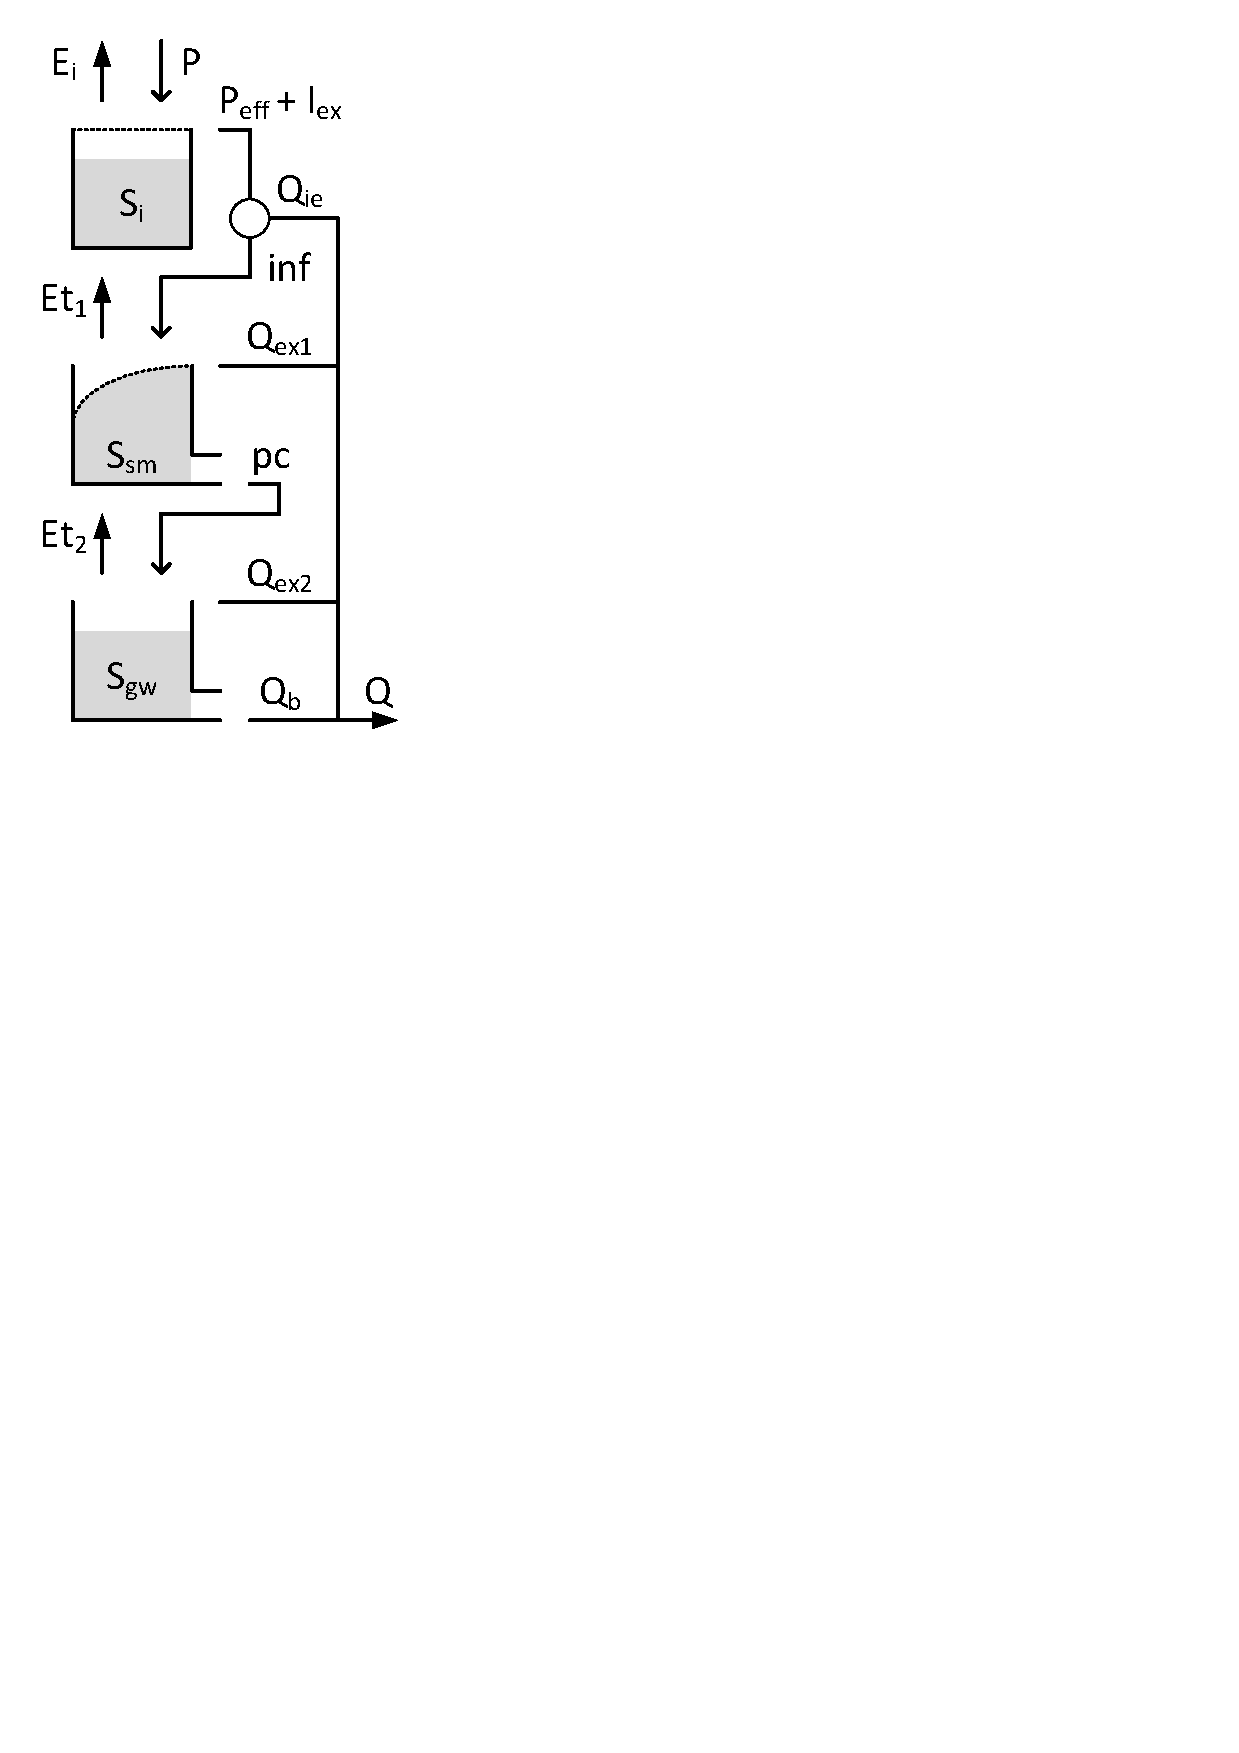
\includegraphics[trim=1cm 17cm 7cm 1cm,width=7cm,keepaspectratio]{./files/22_schematic.pdf}
\caption{Structure of the VIC model} \label{fig:22_schematic}
\end{wrapfigure}

\begin{align}
	\frac{dS_i}{dt} &= P - E_i - P_{eff} - I_{ex} \\
	E_i &= \frac{S_i}{I_{max}}*E_p \\
	I_{max} &= \bar{I}\left(1+I_{\delta}*sin\left(2\pi(t+I_s)\right)\right)\\
	P_eff &=\begin{cases}
		P, & \text{if }S_i = I_{max} \\
		0, & \text{otherwise}\\
	\end{cases}\\
	I_{ex} &= max\left(S_i - I_{max}\right)
\end{align}

Where $S_i$ [mm] is the current interception storage, refilled by precipitation P $[mm/d]$ and drained by evaporation $E_i$ $[mm/d]$ and interception excess flows $P_{eff}$$[mm/d]$ and $I_{ex}$ $[mm/d]$. $E_i$ decreases linearly with storage, based on maximum storage $I_{max}$ [mm]. $I_{max}$ is determined using the mean interception $\bar{I}$ [mm], fractional seasonal interception change $I_{\delta}$ [-] and time shift $I_s$ [d]. It is implicitly assumed that 1 sinusoidal period corresponds with a growing season of 1 year. $P_{eff}$ is effective rainfall when the store is at maximum capacity. $I_{ex}$ is an auxiliary flux used when a change in storage size result in current storage $S_i$ exceeding $I_{max}$.

} % end of wrapfigure fix

\begin{align}
	\frac{dS_{sm}}{dt} &= inf-Et_1-Q_{ex1}-pc\\
	inf &= \left(P_{eff}+I_{ex}\right) - Q_{ie} \\
	Q_{ie} &= \left(P_{eff}+I_{ex}\right)*\left(1-\left(1-\frac{S_{sm}}{S_{sm,max}}\right)^b\right)\\
	E_{t1} &= \frac{S_{sm}}{S_{sm,max}}*(E_p-E_i)\\
	Q_{ex1} &= \begin{cases}
		inf, &\text{if }S_{sm} = S_{sm,max}\\
		0, &\text{otherwise}\\
	\end{cases}	\\
	pc &= k_1*\left(\frac{S_{sm}}{S_{sm,max}}\right)^{c_1}
\end{align}

Where $S_{sm}$ [mm] is the current soil moisture storage, refilled by infiltration $inf$  $[mm/d]$, and drained by evapotranspiration $Et_1$  $[mm/d]$, storage excess $Q_{ex1}$  $[mm/d]$ and percolation $pc$  $[mm/d]$. $inf$ relies on the value of infiltration excess $Q_{ie}$, which is calculated using the maximum soil moisture storage $S_{sm,max}$ [mm] and shape parameter $b$ [-]. $Et_1$ scales linearly with current storage. $Q_{ex1}$ equals $inf$ when the store is at maximum capacity. $pc$ has a potentially non-linear relationship with current storage through time parameter $k_1$ $[d^{-1}]$ and shape parameter $c_1$.

\begin{align}
	\frac{dS_{gw}}{dt} &= pc-Et_2-Q_{ex2}-Q_b\\
	Et_2 &= \frac{S_{gw}}{S_{gw,max}}*\left(E_p-E_i-Et_1\right)\\
	Q_{ex2} &= \begin{cases}
		pc, &\text{if }S_{gw} = S_{gw,max}\\
		0, &\text{otherwise}\\
	\end{cases}	\\
	Q_b &=  k_2*\left(\frac{S_{gw}}{S_{gw,max}}\right)^{c_2}
\end{align}

Where $S_{gw}$ [mm] is the current groundwater storage, refilled through percolation $pc$ $[mm/d]$ and drained by evapotranspiration $Et_2$ $[mm/d]$, excess flow $Q_{ex2}$ $[mm/d]$ and baseflow $Q_b$ $[mm/d]$. $Et_2$ is scaled linearly with current storage based on maximum storage $S_{gw,max}$ [mm]. $Q_{ex2}$ equals $pc$ when the store is at maximum capacity. $Q_b$ has a potentially non-linear relationship with current storage through time parameter $k_2$ and shape parameter $c_2$. Total outflow:

\begin{align}
	Q_t &= Q_{ie}+Q_{ex1}+Q_{ex2}+Q_b
\end{align}

\newpage
\subsubsection{Parameter overview}
% Table generated by Excel2LaTeX from sheet 'Sheet1'
\begin{table}[htbp]
  \centering
    \begin{tabular}{lll}
    \toprule
    Parameter & Unit  & Description \\
    \midrule
    $\bar{I}$ & $mm$  & Mean annual interception storage \\
    $I_{\delta}$ & $-$   & Seasonal interception change as fraction of $\bar{I}$ \\
    $I_s$ & $d$   & Time shift of maximum interception storage \\
    $S_{sm,max}$ & $mm$  & Maximum soil moisture storage \\
    $b$   & $-$   & Shape parameter \\
    $k_1$ & $d^{-1}$ & Runoff coefficient \\
    $c_1$ & $-$   & Runoff nonlinearity \\
    $S_{gw,max}$ & $mm$  & Maximum groundwater storage \\
    $k_2$ & $d^{-1}$ & Runoff coefficient \\
    $c_2$ & $-$   & Runoff nonlinearity \\
    \bottomrule
    \end{tabular}%
  \label{tab:addlabel}%
\end{table}%
